\documentclass[10pt]{article}
\usepackage{fullpage}
\usepackage{graphicx}
\usepackage{amssymb}
\newcommand{\tab}{\hspace*{2em}}
\begin{document}
	\begin{flushright}
	Lindsey Bieda and Joe Frambach\\
	Greedy Algorithm and Dynamic Programming Problems\\
	9.18.2011
	\end{flushright}
	\noindent
	\textbf{(extra credit)} 14. Consider the generalization of the U2 bridge crossing problem where n people with speeds $s_1,\ldots, s_n$
															wish to cross the bridge as quickly as possible. The rules remain:
	
	\begin{itemize}
		\item It is nighttime and you only have one flashlight.
		\item A maximum of two people can cross at any one time
		\item Any party who crosses, either 1 or 2 people must have the ?ashlight with them.
		\item The flashlight must be walked back and forth, it cannot be thrown, etc.
		\item A pair must walk together at the rate of the slower person�s pace.
	\end{itemize}
	
	\noindent
	Give an efficient algorithm to find the fastest way to get a group of people across the bridge.  You
	\textbf{must} have a proof of correctness for your method.\\
	\\
	Algorithm:\\
	Sort the people by speed, increasing, and re-index the array for easy referencing.\\
	$People = [p_1, p_2, \ldots, p_{n-1}, p_n]$, where $p_i < p_j \leftrightarrow s_i < s_j$.\\
	Step 1: Send $p_1$ and $p_2$ across the bridge.\\
	Step 2: Return $p_1$.\\
	Step 3: Send $p_{n-1}$ and $p_n$ across the bridge.\\
	Step 4: Return $p_2$.\\
	The problem is now reduced.\\
	The two slowest people are on the other side. The flashlight is on the starting side.\\
	Repeat the algorithm with input $[p_1, p_2, \ldots, p_{n-3}, p_{n-2}]$.\\
	\\
	Proof:\\
	Assume $\exists$ input $I$ $\ni$ $GRE(I)$ is not correct.\\
	\\
	There are four cases to consider.\\
	\begin{itemize}
	  \item $GRE(I) = [\ldots, (x_k,y_k), \ldots, z, \ldots]$\\
	  $OPT(I) = [\ldots, (x_k,z), \ldots, y_k, \ldots]$, where $OPT$ agrees with GRE for most steps, $k$.\\
	  
	  \item $GRE(I) = [\ldots, (x_k,y_k), \ldots, (w,z) \ldots]$\\
	  $OPT(I) = [\ldots, (x_k,z), \ldots, (v,y_k), \ldots]$, where $OPT$ agrees with GRE for most steps, $k$.\\
	  $OPT^\prime = [\ldots, (x_k,y_k), \ldots, (w,z) \ldots]$.\\
	  GRE defines $x_k > y_k > z$ and $x_k - y_k < x_k - z$.
	  Therefore, $max(x_k,y_k) + z < max(x_k,z) + y_k$, meaning $OPT^\prime$ results in a lower total time than $OPT$.\\
	  
	  \item $GRE(I) = [\ldots, y_k, \ldots, z \ldots]$\\
	  $OPT(I) = [\ldots, z, \ldots, y_k, \ldots]$, where $OPT$ agrees with GRE for most steps, $k$.\\
	  $OPT^\prime = [\ldots, y_k, \ldots, z \ldots]$.\\
	  The total time remains the same. No big deal.\\
	   
	  \item $GRE(I) = [\ldots, y_k, \ldots, (w,z) \ldots]$\\
	  $OPT(I) = [\ldots, z, \ldots, (v,y_k), \ldots]$, where $OPT$ agrees with GRE for most steps, $k$.\\
	\end{itemize}
	In all cases, we create an $OPT^\prime$ such that $OPT^\prime \geq OPT$.\\
	$GRE = \ldots \geq OPT^{\prime\prime} \geq OPT^\prime \geq OPT.~\bot.$
	\\
	
	%answer here
	\newpage
	2. Give a polynomial time algorithm that takes three strings, $A$, $B$ and $C$, as input, and returns the
		 longest sequence $S$ that is a subsequence of $A$, $B$, and $C$.\\
		 %answer here
		\begin{verbatim}
		 3LCS(string A, B, C):
		    return LCS(LCS(A,B), C)
		
		 LCS(string A, B):
		   m = length of A
		   n = length of B
		
		   for i = 1 to m do LCS[i,0] = 0
		   for i = 1 to m do LCS[0,i] = 0
		   
		   for i = 1 to m do:
		       for j = 1 to n do:
		           If A[i] = B[j] then LCS[i,j] = LCS[i-1,j-1] + 1
		           else LCS[i,j] = max(LCS[i-1,j], LCS[i,j-1])
		            
		   return string from traceback 
		\end{verbatim}
		 LCS builds an $n \times n$ table and traceback moves left or up once per iteration. Therefore, we determine
		 that the traceback takes $O(n)$ time and LCS takes $O(n^2)$ time, so our algorithm takes $O(n^2)$ time.\\ 
		 		 
		 \noindent
		 \newpage
	3. Give an efficient algorithm for finding the shortest common super-sequence of two strings $A$ and $B$. $C$
		 is a super-sequence of $A$ if and only if $A$ is a subsequence of $C$.\\
		 HINT: Obviously this problem is very similar to the problem of finding the longest common sub-
		 sequence.   You  should  try  to  first  figure  out  how  to  compute  the  length  of  the  shortest  common
		 super-sequence.
		 \begin{verbatim}
		 SCS(string A, B):
		     m = length of A
		     n = length of B
		     
		     for i = 1 to m do SCS[i,0] = i
		     for i = 1 to n do SCS[0,i] = i
		     
		     for i = 1 to m do:
		         for j = 1 to n do:
		             If A[i] = B[j] then SCS[i,j] = MAX(SCS[i-1][j], SCS[i][j-1])
		             else SCS[i,j] = MIN(SCS[i-1][j], SCS[i][j-1]) + 1
		             
		     return string from traceback
		 \end{verbatim}
		 \newpage
	4. Consider the algorithm that you developed for the previous problem.
	
		\begin{enumerate}
			\item[(a)] Show the table that your algorithm constructs for the inputs $A = zxyyzz$, and $B = zzyxzy$
			\\
			\\
			\begin{tabular}{| c | c | c | c | c | c | c | c | c |}
				\hline
				 & $\epsilon$ & z & x & y & y & z & z\\ \hline
				 $\epsilon$ & 0 & 1 & 2 & 3 & 4 & 5 & 6\\ \hline 
				z & 1 & 1 & 2 & 3 & 4 & 5 & 6\\ \hline
				z & 2 & 2 & 3 & 4 & 5 & 5 & 6\\ \hline
				y & 3 & 3 & 4 & 4 & 5 & 6 & 7\\ \hline
				x & 4 & 4 & 4 & 5 & 6 & 7 & 8\\ \hline
				z & 5 & 5 & 5 & 6 & 7 & 7 & 8\\ \hline
				y & 6 & 6 & 6 & 6 & 7 & 8 & 9\\ \hline 
			\end{tabular}
			\item[(b)] Explain how to find the length of the shortest common super-sequence in your table.\\
			\\ 
			The length for the shortest commen super-sequence is found in the $(length(A), length(B))$ position of the table.
			\item[(c)] Explain how to compute the actual shortest common super-sequence from your table by tracing
								 back from the table entry that gives the length of the shortest common super-sequence.\\
			\begin{verbatim}
			Begin at (i=length(A), j=length(B)) position of the table.
			Prepend the A's ith character to the result.
			While i > 0,
			    If cell value at (i-1,j) < cell value at (i,j), then
			        Set i := i-1.
			        Prepend A's ith character to the result.
			    Else
			        Set i := i-1.
			While j > 0,
			    Prepend B's jth character to the result.
			    Set j := j-1.
			\end{verbatim}
													\begin{figure}[h]
											\centering
												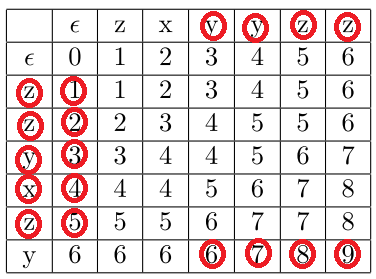
\includegraphics[width=200px]{dynamic4c.png}
											  \caption{Backtracing.}
										\end{figure}
		\end{enumerate}
		% answer here
\end{document}